%----------------------------------------------------------------------------------------
%	COMP 562 Fall 2022 Final Project
%----------------------------------------------------------------------------------------

\documentclass[twoside,twocolumn]{article}

\usepackage{blindtext} % Package to generate dummy text throughout this template 
\usepackage{graphicx}
\usepackage[sc]{mathpazo} % Use the Palatino font
\usepackage[T1]{fontenc} % Use 8-bit encoding that has 256 glyphs
\linespread{1.05} % Line spacing - Palatino needs more space between lines
\usepackage{microtype} % Slightly tweak font spacing for aesthetics

\usepackage[english]{babel} % Language hyphenation and typographical rules?.nb

\usepackage[hmarginratio=1:1,top=32mm,columnsep=20pt]{geometry} % Document margins
\usepackage[hang, small,labelfont=bf,up,textfont=it,up]{caption} % Custom captions under/above floats in tables or figures
\usepackage{booktabs} % Horizontal rules in tables

\usepackage{lettrine} % The lettrine is the first enlarged letter at the beginning of the text

\usepackage{enumitem} % Customized lists
\setlist[itemize]{noitemsep} % Make itemize lists more compact

\usepackage{abstract} % Allows abstract customization
\renewcommand{\abstractnamefont}{\normalfont\bfseries} % Set the "Abstract" text to bold
\renewcommand{\abstracttextfont}{\normalfont\small\itshape} % Set the abstract itself to small italic text

\usepackage{titlesec} % Allows customization of titles
\renewcommand\thesection{\Roman{section}} % Roman numerals for the sections
\renewcommand\thesubsection{\roman{subsection}} % roman numerals for subsections
\titleformat{\section}[block]{\large\scshape\centering}{\thesection.}{1em}{} % Change the look of the section titles
\titleformat{\subsection}[block]{\large}{\thesubsection.}{1em}{} % Change the look of the section titles

\usepackage{fancyhdr} % Headers and footers
\pagestyle{fancy} % All pages have headers and footers
\fancyhead{} % Blank out the default header
\fancyfoot{} % Blank out the default footer
\fancyhead[C]{Running title $\bullet$ May 2016 $\bullet$ Vol. XXI, No. 1} % Custom header text
\fancyfoot[RO,LE]{\thepage} % Custom footer text

\usepackage{titling} % Customizing the title section

\usepackage{hyperref} % For hyperlinks in the PDF

%----------------------------------------------------------------------------------------
%	TITLE SECTION
%----------------------------------------------------------------------------------------

\setlength{\droptitle}{-4\baselineskip} % Move the title up

\pretitle{\begin{center}\Huge\bfseries} % Article title formatting
\posttitle{\end{center}} % Article title closing formatting
\title{Predicting Academic Success Using Multiple Classifier Models} % Article title
\author{% author
\textsc{Amit Parikh} \\[1ex] %\thanks{Corresponding author} \\[1ex] % Your name
\normalsize University of North Carolina at Chapel Hill \\ % Your institution
\normalsize \href{mailto:john@smith.com}{asparikh@live.unc.edu} % Your email address
\and % Uncomment if 2 authors are required, duplicate these 4 lines if more
\textsc{Aryaman Agrawal} \\[1ex] % Your name
\normalsize University of North Carolina at Chapel Hill \\ % Your institution
\normalsize \href{mailto:john@smith.com}{aryamana@live.unc.edu} % Your email address
\and % Uncomment if 2 authors are required, duplicate these 4 lines if more
\textsc{Ernest Ermongkonchai} \\[1ex] % Second author's name
\normalsize University of North Carolina at Chapel Hill \\ % Second author's institution
\normalsize \href{mailto:jane@smith.com}{erneste@email.unc.edu} % Second author's email address
\and % Uncomment if 2 authors are required, duplicate these 4 lines if more
\textsc{Kaan Nymaan} \\[1ex] % Second author's name
\normalsize University of North Carolina at Chapel Hill \\ % Second author's institution
\normalsize \href{mailto:jane@smith.com}{nymanka@email.unc.edu} % Second author's email address
\and % Uncomment if 2 authors are required, duplicate these 4 lines if more
\textsc{Luke Schmidt} \\[1ex] % Second author's name
\normalsize University of North Carolina at Chapel Hill \\ % Second author's institution
\normalsize \href{mailto:jane@smith.com}{lukeant@ad.unc.edu} % Second author's email address
}
\date{\today} % Leave empty to omit a date
\renewcommand{\maketitlehookd}{%
\begin{abstract}
\noindent Classification is one of the fields at the forefront of machine learning research. Our daily lives already use advanced data processing models, whether for identifying spam emails or classifying patient diagnoses. This project utilizes a dataset of students of diverse backgrounds containing both qualitative and quantitative aspects. In this paper, we construct and compare the accuracy to classify students falling above or below average in grades with logistic regression, random forest classifier, and KNN classifier models.%\blindtext % Dummy abstract text - replace \blindtext with your abstract text
\end{abstract}
}

%----------------------------------------------------------------------------------------

\begin{document}
% Print the title
\maketitle

%----------------------------------------------------------------------------------------
%	ARTICLE CONTENTS
%----------------------------------------------------------------------------------------

\section{Introduction}
\subsection{The Data}
\lettrine[nindent=0em,lines=3] {T}he data set used for our research comes from Kaggle and contains information on 650 students in regards to their personal lives and their grades in their Portuguese class. For our model we decided to use a Feature Selection algorithm and ended up using the following features in our model: ‘School’, ‘Sex’, ‘Address’, ‘Mother’s Education’, ‘Father’s Education’, ‘Mother’s Job’, ‘Reason for Choosing School’, ‘Travel Time to School’, ‘Study Time’, ‘Number of Failed Classes’, ‘Amount of Higher Education Classes’, ‘Internet Access’, ‘Schoolday Alcohol Consumption’, ‘Weekend Alcohol Consumption, and Absences’.
\\ \\
The data set was created by Paulo Cortez in the UCI Machine Learning Repository. Each student is binarily classified as an above-average student or a below-average student.
\subsection{Implications}
Our research can be applied to many different school districts and classes across Portugal, providing insight into the feature importance in Portuguese culture. Teachers in these districts can use this model to identify students who may be at risk of under-performance, allowing them to proactively provide the necessary support.

%------------------------------------------------

\section{Framework}

\subsection{Preparing and Exploring the Data}
The general framework of steps that we took are listed below, separated under three primary categories: Preparing \& Exploring the Data, Building the Classifier Models, and Evaluating Model Results. 
\begin{enumerate}
	\item We downloaded the Portuguese.csv file from Kaggle and read it into our notebook
	\item Calculated the median final grade among students in our dataset
	\item Used this median to create a binary target variable representing if a student earns an above or below average grade
	\item Encoded all categorical features as numeric using one-hot encoding 
	\item Selected the top 15 features by their ANOVA F-value, eliminating features that were not relevant to the model
	\item Visualized the distributions and covariance matrix of our selected features to ensure the input data was statistically sound and had low multi-collinearity
	\item Split the data into training and testing sets using a 75/25 split. It is industry standard, and is a good split to avoid over-fitting
\end{enumerate}

\subsection{Building the Classifier Models}
These general steps were applied to each of the three classification models we compared:
\begin{enumerate}
	\item Create classification model object (Logistic Regression, Random Forest, or KNN)
	\item Build a grid of hyper-parameters and tune these during Cross Validation
	\item Fit the model using the X and y training data
\end {enumerate}

\subsection{Evaluating Model Results}
These general steps were applied to each of the three classification models we compared:
\begin{enumerate}
	\item Make predictions using each of the trained models
	\item Calculate accuracy of predictions using the Jaccard similarity index for in and out of sample data
	\begin{equation}
	\label{eq:emc}
	J(A,B) = \frac{|{A}\cap{B}|}{|{A}\cup{B}|}
	\end{equation}
	\item Model predictions into a confusion matrix to better understand the strengths and weaknesses of our model’s predictive power
	\item Find feature importance of our finalized model to analyze and interpret the meaning from our model
\end {enumerate}

%Text requiring further explanation\footnote{Example footnote}.

%------------------------------------------------

\section{Building the Model}
Once our Kaggle dataset is loaded, we utilize several classifier models to predict students’ performance in the classroom. We will test three different models in order to compare the accuracy of each and find a better solution for our prediction. 
\\ \\
After training each of our models with the full dataset containing 30 features (including birth, sex, housing, etc.), we realized that this would cause our final prediction to overfit our training data. This is because we saw that some variables were highly correlated with each other from calculating a covariance matrix with all 30 features. With this information at hand, we were able to use a feature selection algorithm that removed half of the unneeded correlated features. This was done by taking the top 15 features by their ANOVA F-value. Making this adjustment significantly improved our prediction accuracy as indicated by our confusion matrix.

\subsection{Logistic Regression}
The purpose of using the logistic regression model is to have a baseline classification model which is simple to implement and an effective way to check whether other models meet the performance and accuracy expectations.
\\ \\
A logistic model takes the multiple features and uses a sigmoid function to squash the results into the [0, 1] range. This is an example of binary logistic regression which will be able to predict an above-average grade (1) and a below-average grade (0), where the parameters are:
\\ \\
$p(y|\textbf{x},\beta_{0},\beta)=\frac{1}{1+exp\{-y(\beta_{0}+\textbf{x}^T\beta)\}}$
\\ \\
From cross validation we found that the optimal hyperparameters are C = 1 and a penalty = none. C tells the model how much weight to give to the training data and the penalty hurts models with more variables if present.

\subsection{Random Forrest Classifier}
Random Forest is one of the most popular and powerful classification algorithms because of its similarity to human-like thinking which leads to high intuition and interpretability.
\\ \\
A Random Forest classifier is an ensembling technique consisting of many decision trees. It builds an independent set of trees which classify inputs by voting on outcomes - an approach that is more accurate than individual trees. 
\\ \\
Cross validation yielded an optimal max depth of 3 and 166 for n\_estimators. The max depth represents the number of splits the model can make. N\_estimators is the number of trees to build before averaging the predictions. 

\subsection{KNN Classifier}
The purpose of using the KNN model, just like the Logistic Regression, is for its simplicity and accuracy and is an effective way to check the other models.
\\ \\
A KNN classifier is a supervised learning classifier, which uses proximity to make classifications or predictions about the grouping of individual data points. This model works off the assumption that similar points are in close proximity to each other.
\\ \\
$D(X,Y)=(\sum_{i=1}^{n}|x_i-y_i|^p)^{\frac{1}{p}}$
\\ \\
Using the Minkowski distance formula used above for the data points and cross validation, the optimal number of nearest neighbors to use was found to be 14. 

%------------------------------------------------

\section{Results}
The random forest classifier was found to be the most accurate machine learning model we trained, achieving an accuracy rate of 74.8\% on our validation set and 76.5\% on our training set. 74.8\% was the highest out-of-sample accuracy rate in comparison to other models such as logistic regression (72.3\%), and k nearest neighbors (68.7\%).
\begin{figure}
  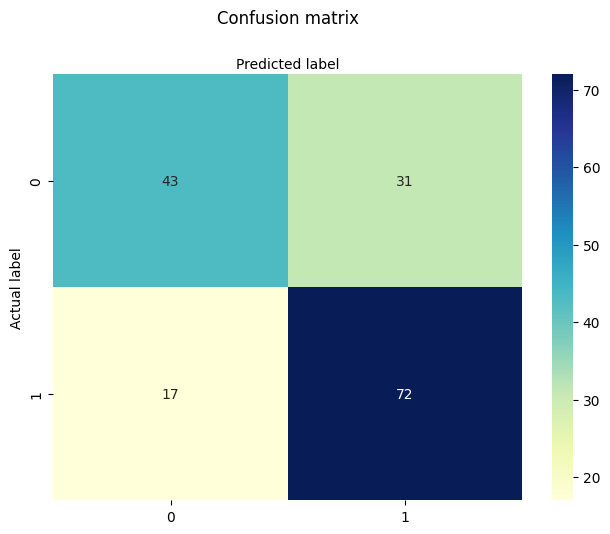
\includegraphics[width=\linewidth]{confusion_matrix.png}
  \caption{Confusion matrix for Random Forest Model}
  \label{fig:matrix}
\end{figure}
%Figure \ref{fig:matrix} shows a boat.
\\ \\
The results of the confusion matrix showed that while the random forest classifier was able to accurately measure and predict positive cases, it was not as successful in accurately predicting and measuring negative cases. This suggests that further fine-tuning and optimization of the model may be necessary in order to improve its accuracy in negative cases as the false positives is as high as 35.
\\ \\
The most important factor in predicting student performance, as determined by the mean decrease in impurity (MDI) method, was found to be failing a prior class. This was followed by seeking higher education, mother's education and job, school, weekly study time, father's education, and internet access, among other factors. Collectively, these were judged to be the most influential components of student performance.
\begin{figure}
  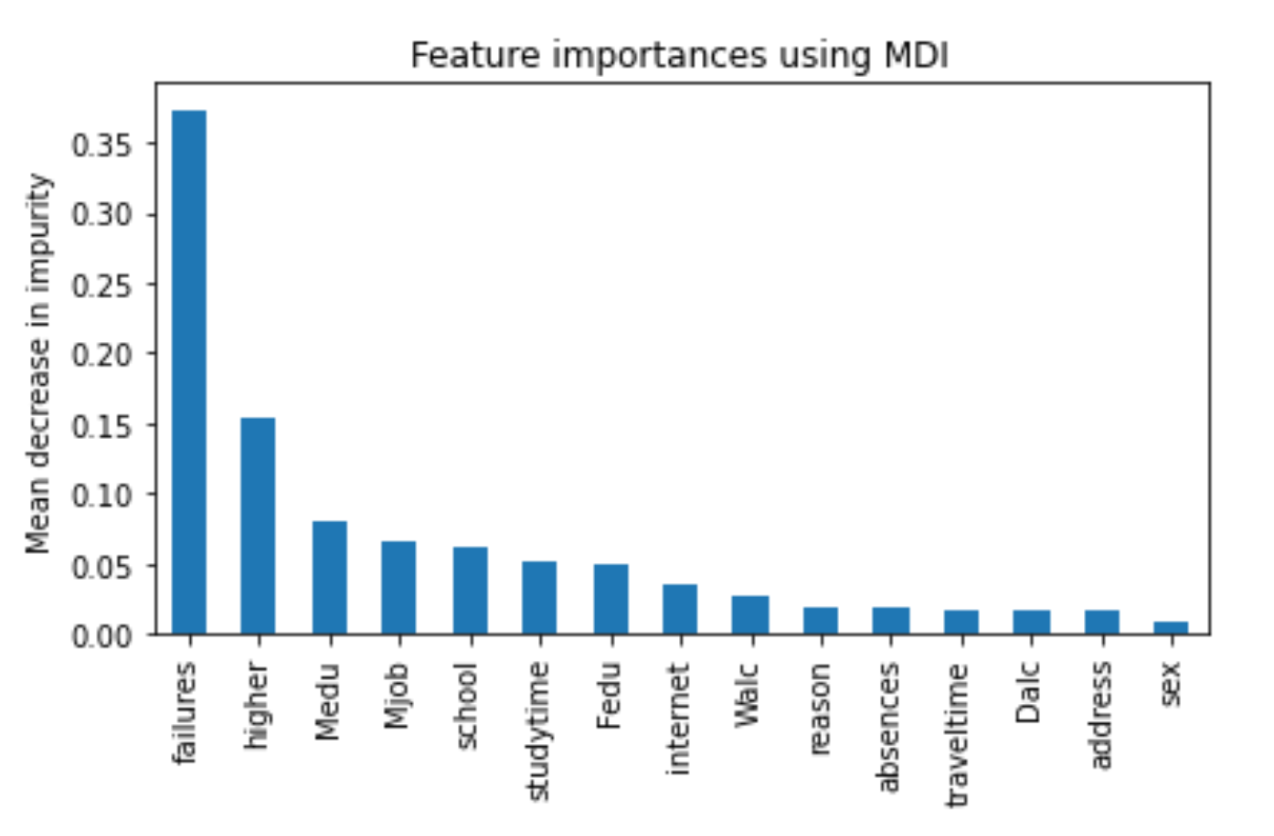
\includegraphics[width=\linewidth]{importance.png}
  \caption{Feature Importances Using MDI}
  \label{fig:imp}
\end{figure}
%------------------------------------------------

\section{Conclusion}
Even though our results were fairly accurate, it could be significantly improved through the use of a larger data set or a more robust set of features. While our general framework could be applied to other schools and countries, we cannot use the same set of features for just any country or subject. This is because academic performance is also reliant on factors such as culture and the importance placed on academics in other countries. Our study can be enhanced by using the same framework in multiple countries and schools to gain a better understanding of what factors influence academic success.

%----------------------------------------------------------------------------------------
%	REFERENCE LIST
%----------------------------------------------------------------------------------------

\begin{thebibliography}{99} % Bibliography - this is intentionally simple in this template
\bibitem{}LynnSpeiserPersonEnvelope, Jaime, and Michael E.MillerEnvelope. “A Comparison of Random Forest Variable Selection Methods for Classification Prediction Modeling.” Expert Systems with Applications, Pergamon, 23 May 2019, https://www.sciencedirect.com

\bibitem{}Rao, Medabalimi. “Texture Classification Using Minkowski Distance Measure-Based Clustering for Feature Selection.”, https://www.spiedigitallibrary.org/journal-of-electronic-imaging. Accessed 9 Dec. 2022.

\bibitem{}“Alcohol Effects On Study | Kaggle.” Kaggle: Your Machine Learning and Data Science Community, https://www.kaggle.com/datasets/whenam ancodes/alcohol-effects-on-study Accessed 9 Dec. 2022.
\end{thebibliography}

%----------------------------------------------------------------------------------------
%------------------------------------------------
% EXTRA
%------------------------------------------------

%\section{Results}
%
%\begin{table}
%\caption{Example table}
%\centering
%\begin{tabular}{llr}
%\toprule
%\multicolumn{2}{c}{Name} \\
%\cmidrule(r){1-2}
%First name & Last Name & Grade \\
%\midrule
%John & Doe & $7.5$ \\
%Richard & Miles & $2$ \\
%\bottomrule
%\end{tabular}
%\end{table}
%
%\blindtext % Dummy text
%
%\begin{equation}
%\label{eq:emc}
%e = mc^2
%\end{equation}
%
%\blindtext % Dummy text
%
%%------------------------------------------------
%
%\section{Discussion}
%
%\subsection{Subsection One}
%
%A statement requiring citation \cite{Figueredo:2009dg}.
%\blindtext % Dummy text
%
%\subsection{Subsection Two}
%
%\blindtext % Dummy text
%------------------------------------------------
% EXTRA
%------------------------------------------------
\end{document}
